%\section{Audio Clean-up by AudioSep}
%To address the longer audio in the data that prevented Audiosep from being used, we start by cutting shorter audio clips with low-threshold~(less than 0.05) PANNs.
%

%\begin{figure}[th]
%	\scalebox{0.5}{\includegraphics{words2/leftByWord/9-16.png}}
%	\caption{9-16left: may about eating and food}}
%	\label{fig:9-16}
%\end{figure}


%
%\section{Phonemes Information}
%
%\begin{table}[th]
%\centering
%\small
%\begin{tabular}{lcc}
%\hline
%\textbf{Phoneme} & \textbf{Mean Length} & \textbf{Variance of Length}\\
%\hline
%\verb|0| & 0.0569 & 0.0009 \\
%\verb|1| & 0.1031 & 0.0085 \\
%\verb|2| & 0.0927 & 0.0098 \\
%\verb|3| & 0.1224 & 0.0181 \\
%\verb|4| & 0.0873 & 0.0063 \\
%\verb|5| & 0.0413 & 0.0008 \\
%\verb|6| & 0.1033 & 0.0152 \\
%\verb|7| & 0.0837 & 0.0054 \\
%\verb|8| & 0.0916 & 0.0082 \\
%\verb|9| & 0.1253 & 0.0239 \\
%\verb|10| & 0.1045 & 0.0097 \\
%\verb|11| & 0.0934 & 0.0057 \\
%\verb|12| & 0.2063 & 0.0690 \\
%\verb|13| & 0.0983 & 0.0104 \\
%\verb|14| & 0.1275 & 0.0189 \\
%\verb|15| & 0.1070 & 0.0150 \\
%\verb|16| & 0.0944 & 0.0058 \\
%\verb|17| & 0.1018 & 0.0092 \\
%\verb|18| & 0.0737 & 0.0046 \\
%\verb|19| & 0.1602 & 0.0279 \\
%\verb|20| & 0.0787 & 0.0035 \\
%\verb|21| & 0.1685 & 0.0399 \\
%\verb|22| & 0.0878 & 0.0073 \\
%\verb|23| & 0.0933 & 0.0070 \\
%\verb|24| & 0.0960 & 0.0046 \\
%\verb|25| & 0.1313 & 0.0213 \\
%\verb|26| & 0.1075 & 0.0115 \\
%\verb|27| & 0.1387 & 0.0229 \\
%\verb|28| & 0.1017 & 0.0082 \\
%\verb|29| & 0.0931 & 0.0111 \\
%\verb|30| & 0.1018 & 0.0120 \\
%\verb|31| & 0.2208 & 0.0786 \\
%\verb|32| & 0.2002 & 0.0576 \\
%\verb|33| & 0.0655 & 0.0016 \\
%\verb|34| & 0.0826 & 0.0102 \\
%\verb|35| & 0.0479 & 0.0008 \\
%\verb|36| & 0.0689 & 0.0018 \\
%\verb|37| & 0.1820 & 0.0526 \\
%\verb|38| & 0.0750 & 0.0041 \\
%\verb|39| & 0.0947 & 0.0104 \\
%\verb|40| & 0.0342 & 0.0002 \\
%\verb|41| & 0.1187 & 0.0189 \\
%\verb|42| & 0.0766 & 0.0017 \\
%\verb|43| & 0.1613 & 0.0312 \\
%\verb|44| & 0.1183 & 0.0069 \\
%\verb|45| & 0.1223 & 0.0254 \\
%\verb|46| & 0.0705 & 0.0018 \\
%\verb|47| & 0.1089 & 0.0127 \\
%\verb|48| & 0.2405 & 0.0709 \\
%\verb|49| & 0.1162 & 0.0211 \\\hline
%\end{tabular}
%\caption{Mean Length and Variance of Length for each phoneme}
%\label{tab:mlvl}
%\end{table}
%
%\begin{table}[h]
%\centering
%\begin{tabular}{llllll}
%\hline
%\textbf{2-gram} & \textbf{Popularity Score} & \textbf{3-gram} & \textbf{Popularity Score} & \textbf{4-gram} & \textbf{Popularity Score} \\ \hline
%\verb|[35, 40]| & 1.0638 & [35, 40, 33] & 0.3211 & [40, 33, 34, 44] & 0.1096 \\
%\verb|[40, 33]| & 0.5462 & [40, 33, 34] & 0.1861 & [35, 40, 33, 34] & 0.0987 \\
%\verb|[18, 5]| & 0.3350 & [35, 40, 0] & 0.1840 & [35, 40, 33, 16] & 0.0656 \\
%\verb|[33, 34]| & 0.3129 & [33, 34, 44] & 0.1625 & [35, 40, 0, 42] & 0.0477 \\
%\verb|[34, 44]| & 0.2926 & [40, 33, 16] & 0.1083 & [40, 33, 16, 34] & 0.0355 \\
%\verb|[5, 40]| & 0.2917 & [0, 42, 20] & 0.0990 & [35, 0, 42, 20] & 0.0320 \\
%\verb|[20, 23]| & 0.2764 & [8, 35, 40] & 0.0971 & [35, 40, 0, 33] & 0.0298 \\
%\verb|[2, 5]| & 0.2424 & [35, 40, 16] & 0.0757 & [35, 40, 16, 11] & 0.0252 \\
%\verb|[23, 18]| & 0.2276 & [18, 35, 40] & 0.0632 & [8, 35, 40, 33] & 0.0240 \\
%\verb|[35, 0]| & 0.2261 & [5, 40, 33] & 0.0628 & [0, 42, 20, 23] & 0.0239 \\
%\verb|[40, 0]| & 0.2257 & [40, 0, 42] & 0.0602 & [40, 0, 42, 20] & 0.0238 \\
%\verb|[6, 5]| & 0.2231 & [33, 16, 34] & 0.0596 & [35, 40, 33, 41] & 0.0222 \\
%\verb|[22, 5]| & 0.2208 & [35, 0, 42] & 0.0557 & [40, 33, 16, 11] & 0.0209 \\
%\verb|[5, 14]| & 0.2203 & [35, 5, 40] & 0.0541 & [33, 16, 34, 44] & 0.0174 \\
%\verb|[29, 18]| & 0.2144 & [35, 40, 24] & 0.0536 & [33, 34, 44, 4] & 0.0168 \\
%\verb|[36, 29]| & 0.2127 & [40, 33, 41] & 0.0525 & [5, 40, 33, 34] & 0.0163 \\
%\verb|[8, 35]| & 0.2103 & [40, 16, 11] & 0.0524 & [18, 35, 40, 33] & 0.0155 \\
%\verb|[5, 18]| & 0.2101 & [2, 35, 40] & 0.0504 & [15, 35, 40, 33] & 0.0150 \\
%\verb|[15, 5]| & 0.2048 & [27, 9, 20] & 0.0496 & [35, 40, 33, 42] & 0.0148 \\
%\verb|[5, 22]| & 0.2044 & [14, 35, 40] & 0.0466 & [35, 5, 40, 33] & 0.0135 \\
%\verb|[16, 11]| & 0.2030 & [42, 20, 23] & 0.0457 & [41, 27, 9, 20] & 0.0114 \\
%\verb|[5, 26]| & 0.1953 & [36, 29, 18] & 0.0438 & [0, 33, 34, 44] & 0.0110 \\
%\verb|[9, 20]| & 0.1932 & [35, 40, 42] & 0.0437 & [14, 35, 40, 33] & 0.0107 \\
%\verb|[27, 9]| & 0.1931 & [41, 27, 9] & 0.0424 & [33, 34, 44, 23] & 0.0106 \\
%\verb|[0, 42]| & 0.1931 & [6, 35, 40] & 0.0393 & [40, 0, 33, 34] & 0.0094 \\
%\verb|[13, 5]| & 0.1920 & [15, 35, 40] & 0.0391 & [5, 40, 33, 16] & 0.0091 \\
%\verb|[5, 46]| & 0.1747 & [26, 35, 40] & 0.0389 & [35, 40, 33, 27] & 0.0091 \\
%\verb|[26, 5]| & 0.1731 & [35, 40, 1] & 0.0384 & [6, 35, 40, 33] & 0.0091 \\
%\verb|[42, 20]| & 0.1723 & [9, 32, 20] & 0.0376 & [8, 35, 40, 0] & 0.0089 \\
%\verb|[5, 36]| & 0.1658 & [22, 35, 40] & 0.0367 & [35, 40, 16, 34] & 0.0088 \\
%% Add more rows as needed
%\hline
%\end{tabular}
%\caption{Selected words in vocabulary with popularity score.}
%\label{table:your_table_label}
%\end{table}

\section{Probabilistic Context-Free Grammars and Adaptor Grammars}
\label{sec:pcfg}
Probabilistic Context-free Grammars (PCFGs)~\citep{manning1999foundations} are an extension of context-free grammars that assign a probability to each production rule, providing a probabilistic framework for generating strings.
A PCFG is defined as a tuple $(N, \Sigma, R, S, P)$ where $N$ is a set of non-terminal symbols, $\Sigma$ is a set of terminal symbols, $R$ is a set of production rules of the form $A \rightarrow \beta$, $S$ is the start symbol, and $P(A \rightarrow \beta)$ is the probability associated with the production rule $A \rightarrow \beta$ such that $\sum_{\beta} P(A \rightarrow \beta) = 1$ for all $A \in N$.

The adapted tree distributions $H_{n}$ is generated by using a \textit{Pitman-Yor process}~\citep{pitman1997two},
a generalization of Dirichlet process~\citep{ferguson1973bayesian}. A draw $H_{n} \equiv (\pi_{n}, z_{n})$ is formed by the stick breaking process~\citep{sudderth2008shared} parametrized by scale parameter $a$, discount factor $b$, and base distribution $G_{n}$:
\begin{multline}
{\pi\prime}_{k} \sim \text{Beta}(1-b, a+kb), \; z_{k} \sim G_{n} \\
{\pi}_{k} \equiv {\pi\prime}_{k} {\textstyle \prod_{k-1}^{j=1}} (1- {\pi\prime}_{j}), \; H\equiv{\textstyle \sum_{k}^{}} \pi_{k}\delta_{z_{k}}
\end{multline}

\begin{algorithm}[h]
        \scriptsize
        \caption{Parse Algorithm}\label{alg:pa}
        \begin{algorithmic}[1]
                \State For nonterminals $e \in N$, draw rule probabilities $p_{e} \sim Dir(\alpha_{n})$ for PCFG $G$
                \For{adapted nonterminal $n$}
                \State Draw $H_{n} \sim \text{PYGEM}(a_{n}, b_{n}, G_{n})$ according to Equation 1, where $G_{n}$ is defined by the PCFG rules $R$.
                \EndFor
                \State For $i \in {1, ..., D}$, generate a hierarchical structure tree $t_{s, i}$ using the PCFG rules $R(e)$ at non-adapted nonterminal e and the $H_{c}$ at adapted nonterminals n.
                \State The yields of trees $t1, ..., t_{D}$ are observations $x_{1}, ..., x_{D}$.

        \end{algorithmic}
\end{algorithm}

\section{Causal strength of top 35 words}
\label{sec:top}
Here are the causal strength for the top 35 words and activities.

\begin{figure*}[ht]
	\centering
%	\ContinuedFloat
		\begin{minipage}[b]{.3\linewidth}
			\centering
			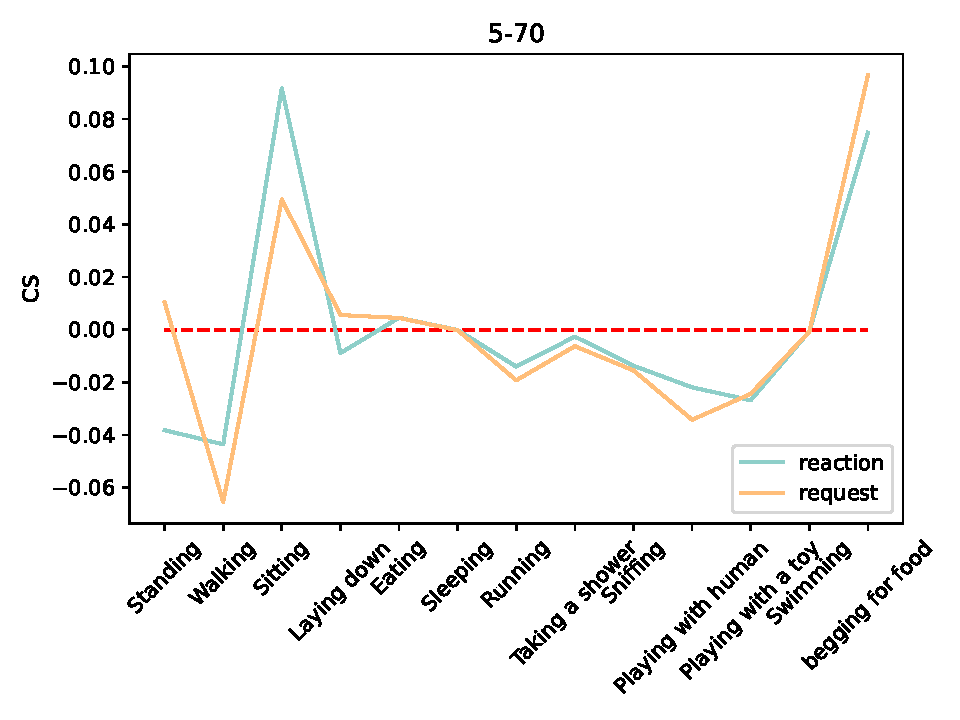
\includegraphics[width=0.99\linewidth]{./35word/5-70.pdf}
		\end{minipage}
		\begin{minipage}[b]{.3\linewidth}
			\centering
			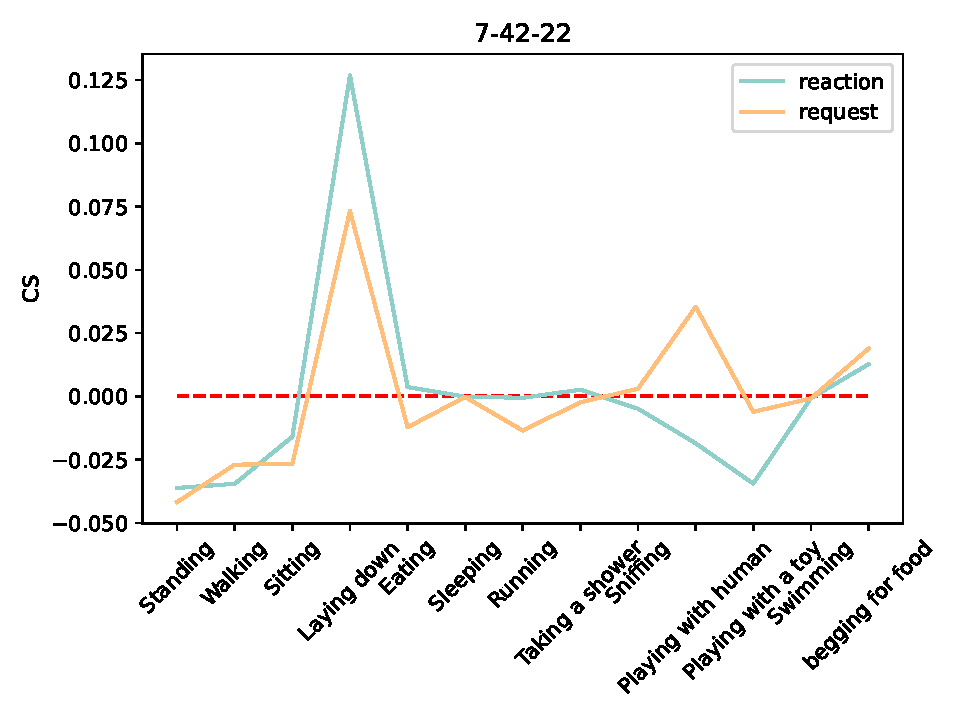
\includegraphics[width=0.99\linewidth]{./35word/7-42-22.pdf}
		\end{minipage}
		\begin{minipage}[b]{.3\linewidth}
			\centering
			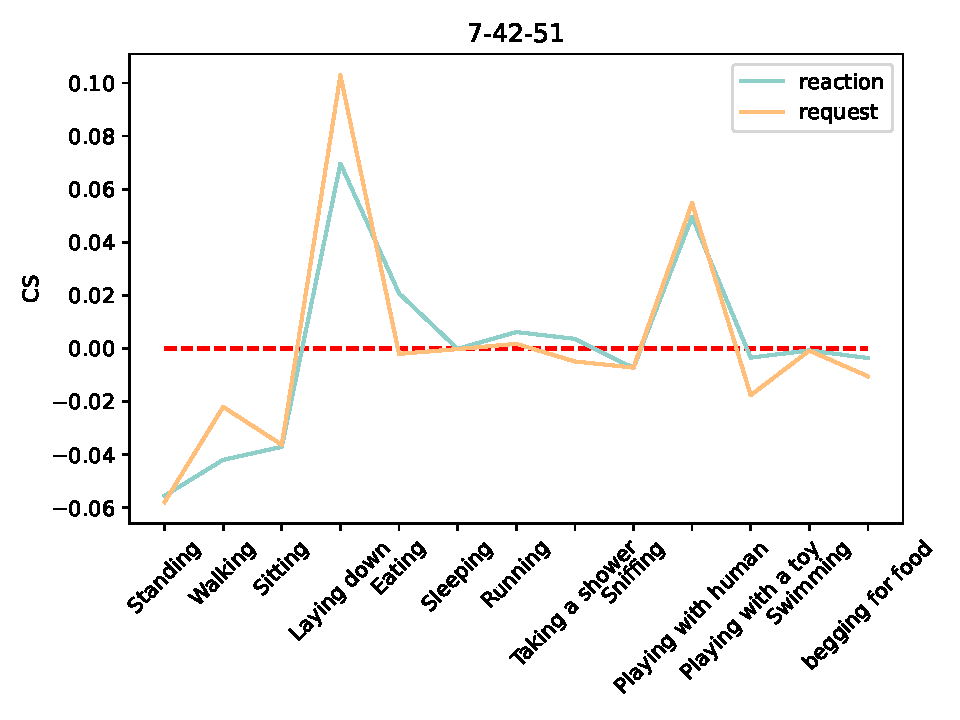
\includegraphics[width=0.99\linewidth]{./35word/7-42-51.pdf}
		\end{minipage}

		\begin{minipage}[b]{.3\linewidth}
			\centering
			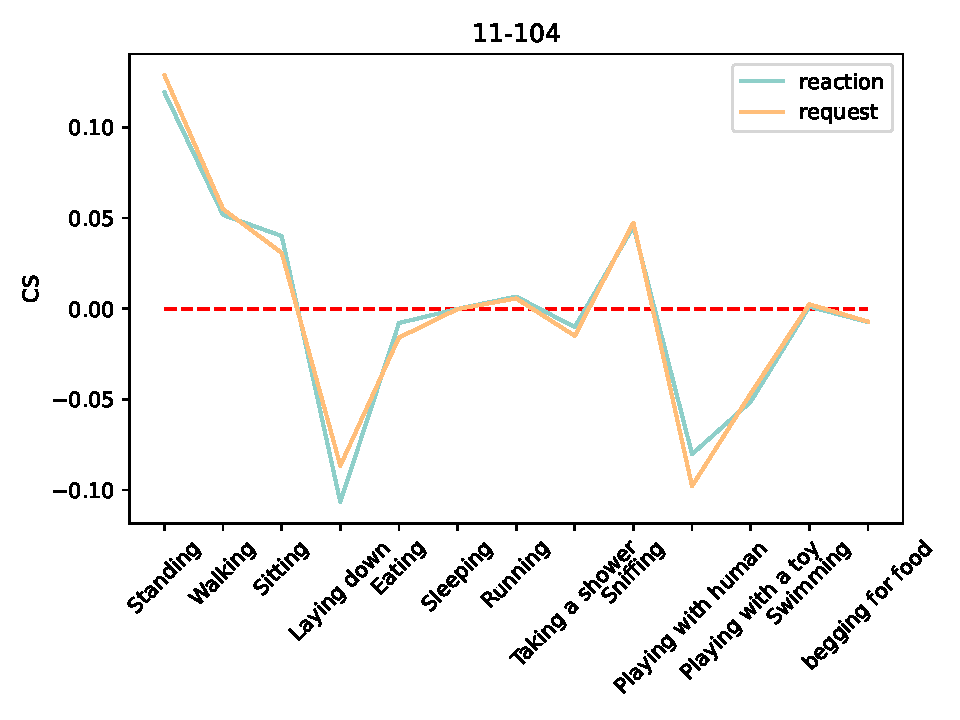
\includegraphics[width=0.99\linewidth]{./35word/11-104.pdf}
		\end{minipage}
		\begin{minipage}[b]{.3\linewidth}
			\centering
			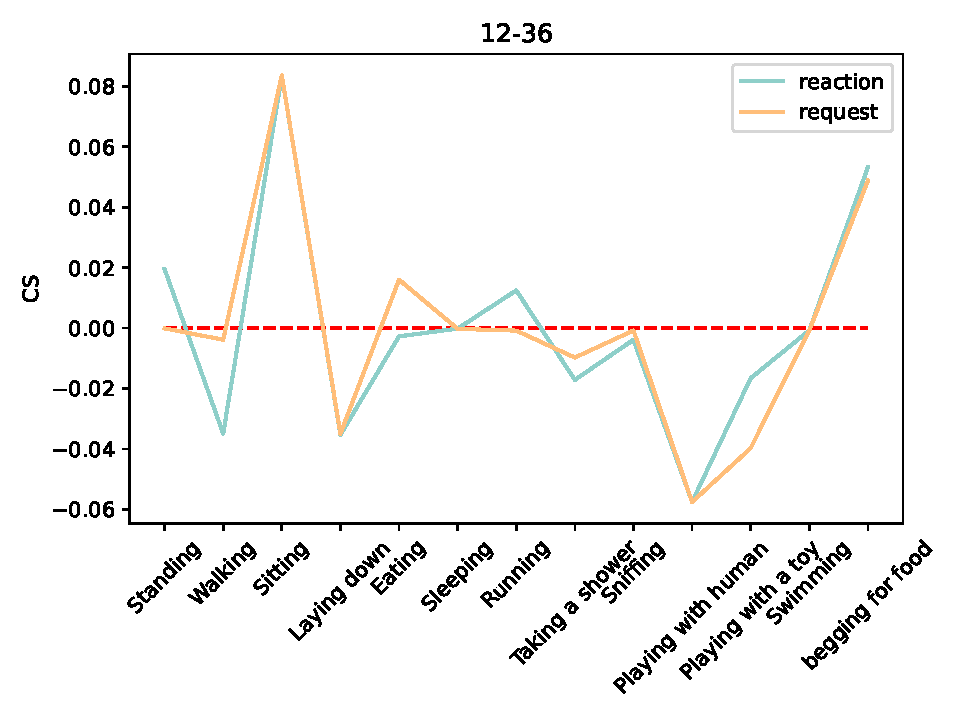
\includegraphics[width=0.99\linewidth]{./35word/12-36.pdf}
		\end{minipage}
		\begin{minipage}[b]{.3\linewidth}
			\centering
			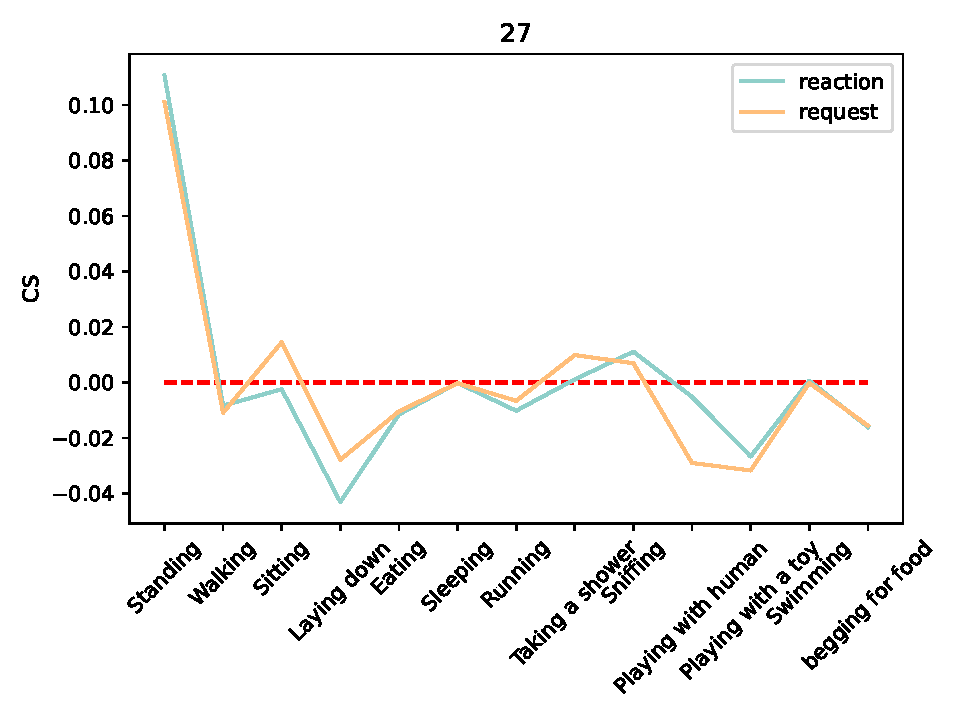
\includegraphics[width=0.99\linewidth]{./35word/27.pdf}
		\end{minipage}
		
				\begin{minipage}[b]{.3\linewidth}
			\centering
			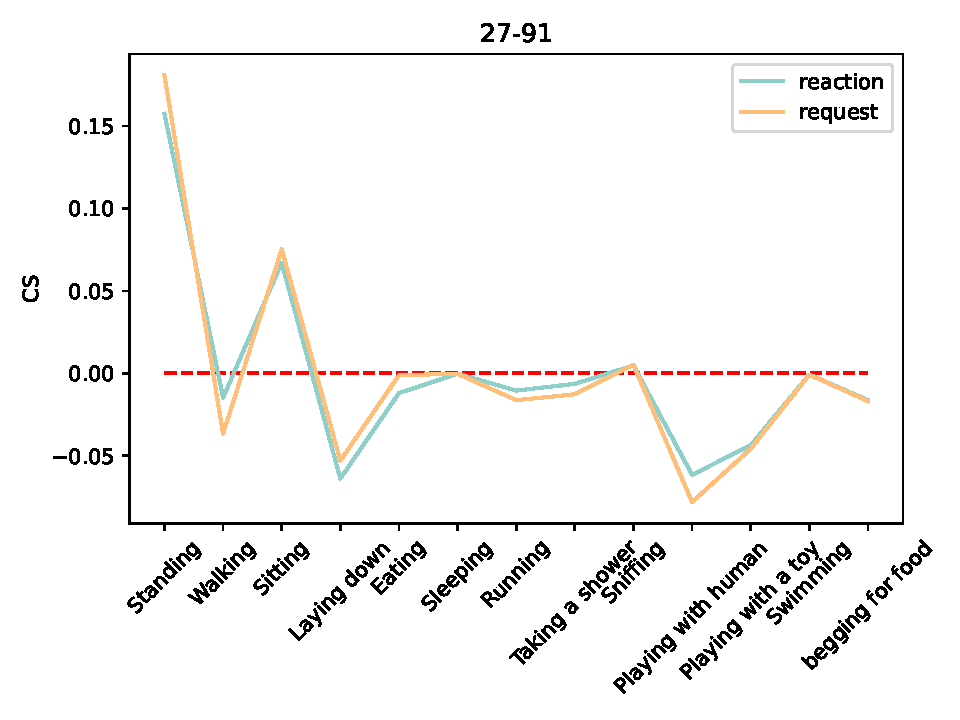
\includegraphics[width=0.99\linewidth]{./35word/27-91.pdf}
		\end{minipage}
		\begin{minipage}[b]{.3\linewidth}
			\centering
			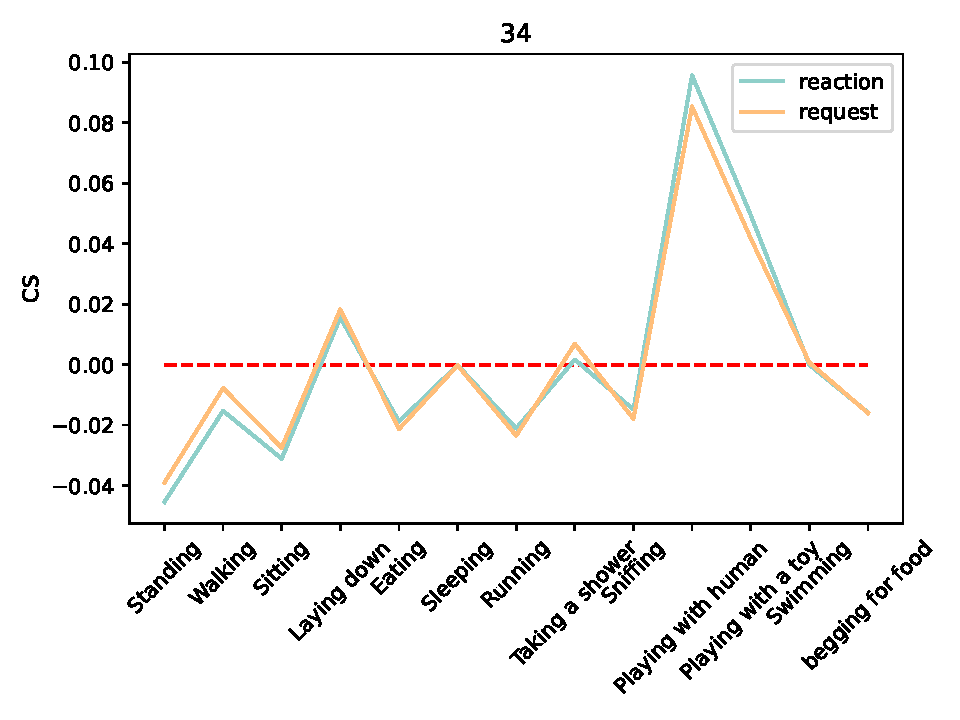
\includegraphics[width=0.99\linewidth]{./35word/34.pdf}
		\end{minipage}
		\begin{minipage}[b]{.3\linewidth}
			\centering
			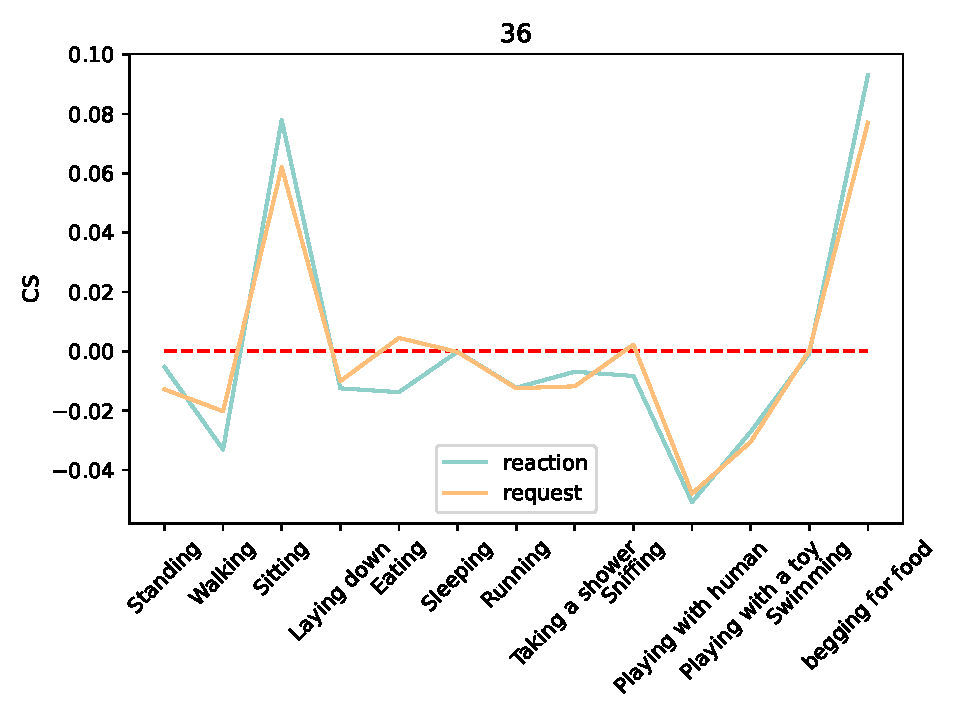
\includegraphics[width=0.99\linewidth]{./35word/36.pdf}
		\end{minipage}
		
		\begin{minipage}[b]{.3\linewidth}
			\centering
			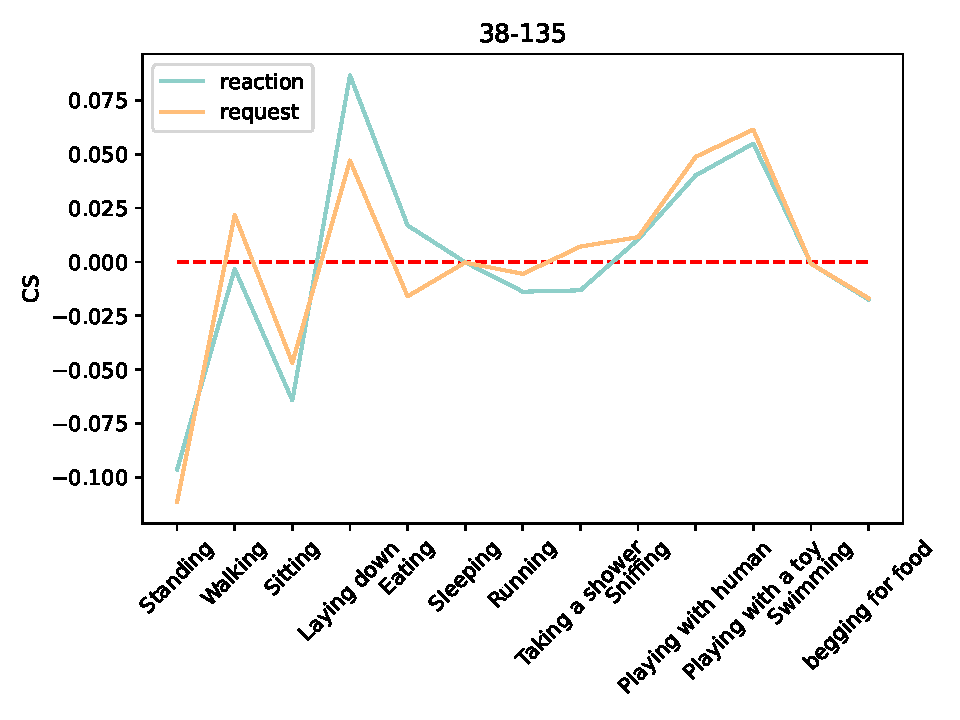
\includegraphics[width=0.99\linewidth]{./35word/38-135.pdf}
		\end{minipage}
		\begin{minipage}[b]{.3\linewidth}
			\centering
			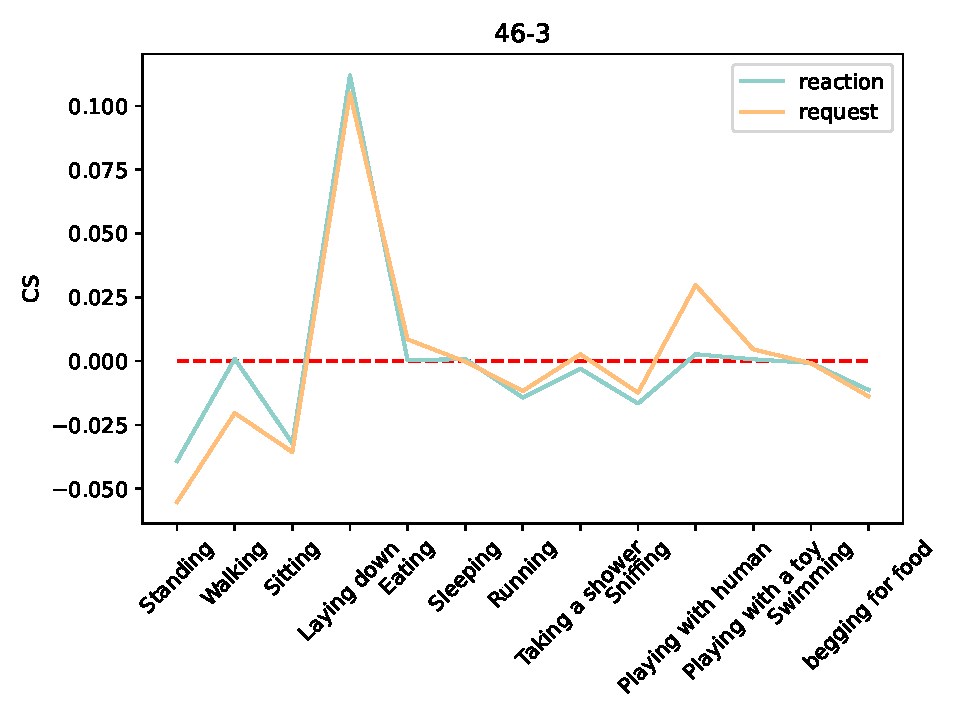
\includegraphics[width=0.99\linewidth]{./35word/46-3.pdf}
		\end{minipage}
		\begin{minipage}[b]{.3\linewidth}
			\centering
			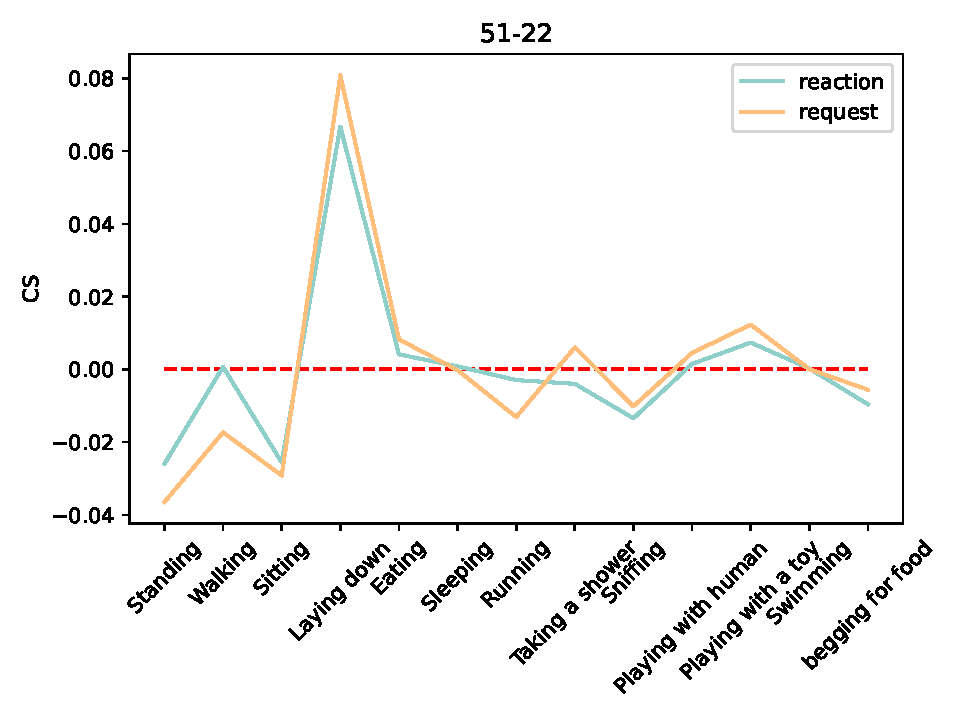
\includegraphics[width=0.99\linewidth]{./35word/51-22.pdf}
		\end{minipage}
		
				\begin{minipage}[b]{.3\linewidth}
			\centering
			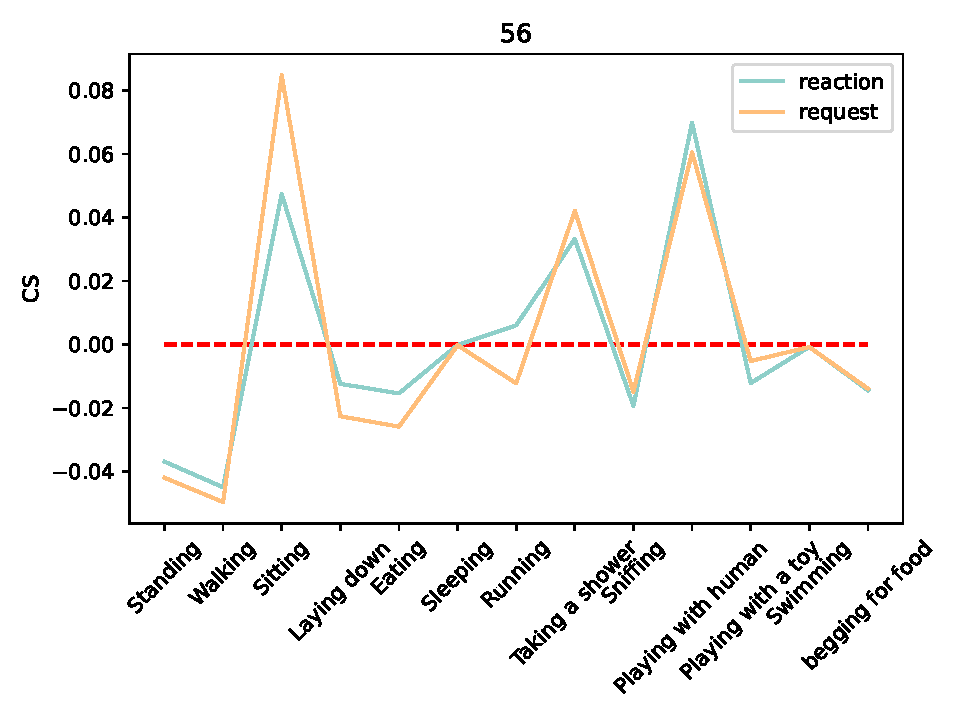
\includegraphics[width=0.99\linewidth]{./35word/56.pdf}
		\end{minipage}
		\begin{minipage}[b]{.3\linewidth}
			\centering
			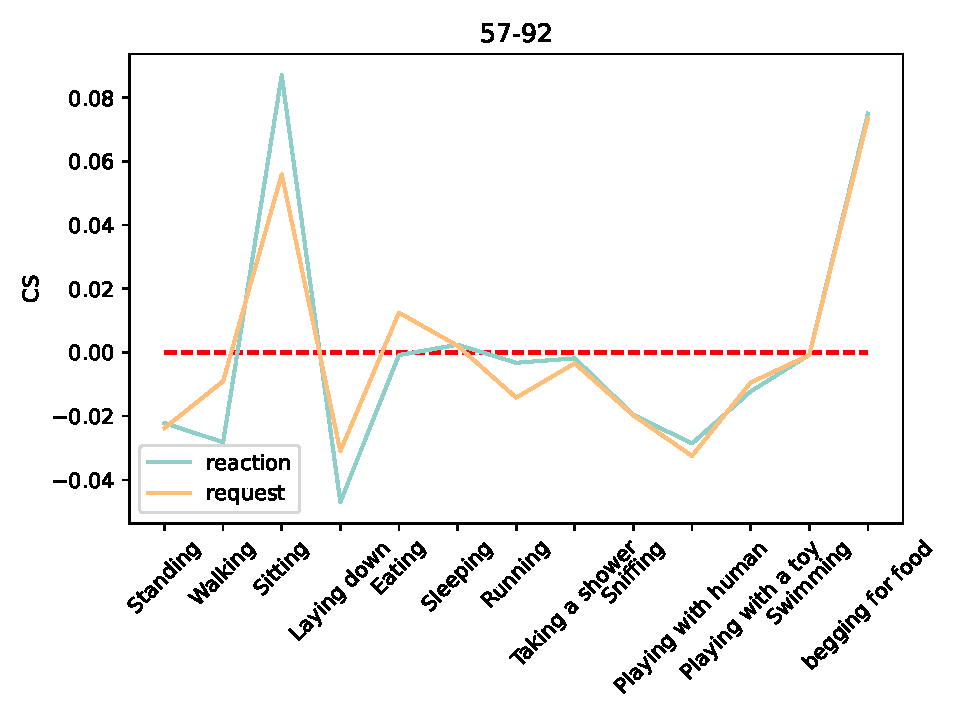
\includegraphics[width=0.99\linewidth]{./35word/57-92.pdf}
		\end{minipage}
		\begin{minipage}[b]{.3\linewidth}
			\centering
			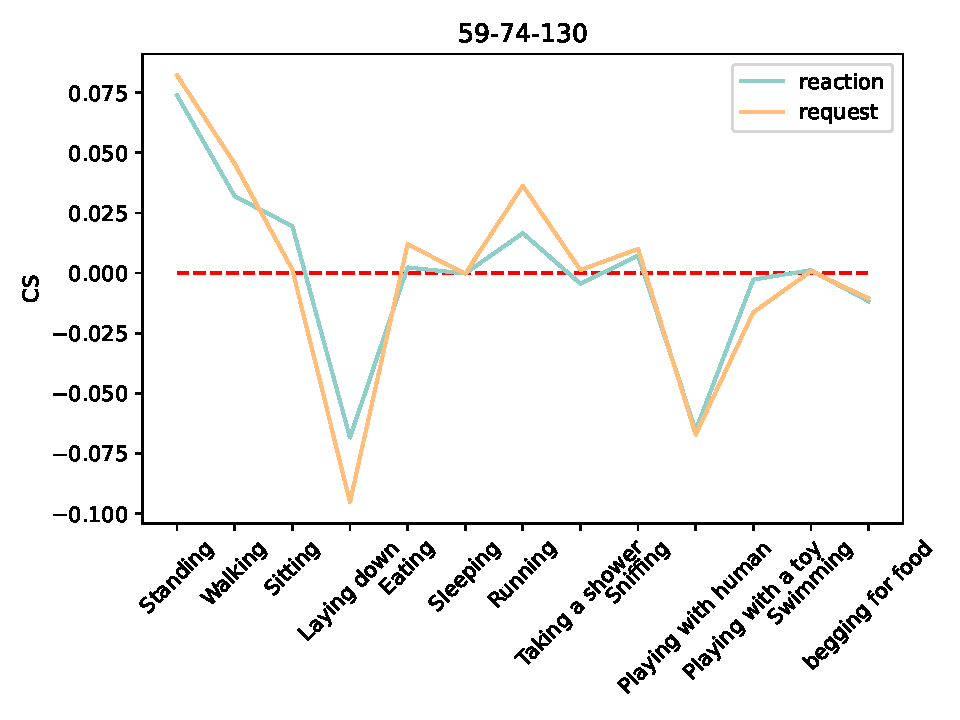
\includegraphics[width=0.99\linewidth]{./35word/59-74-130.pdf}
		\end{minipage}
		
		\begin{minipage}[b]{.3\linewidth}
			\centering
			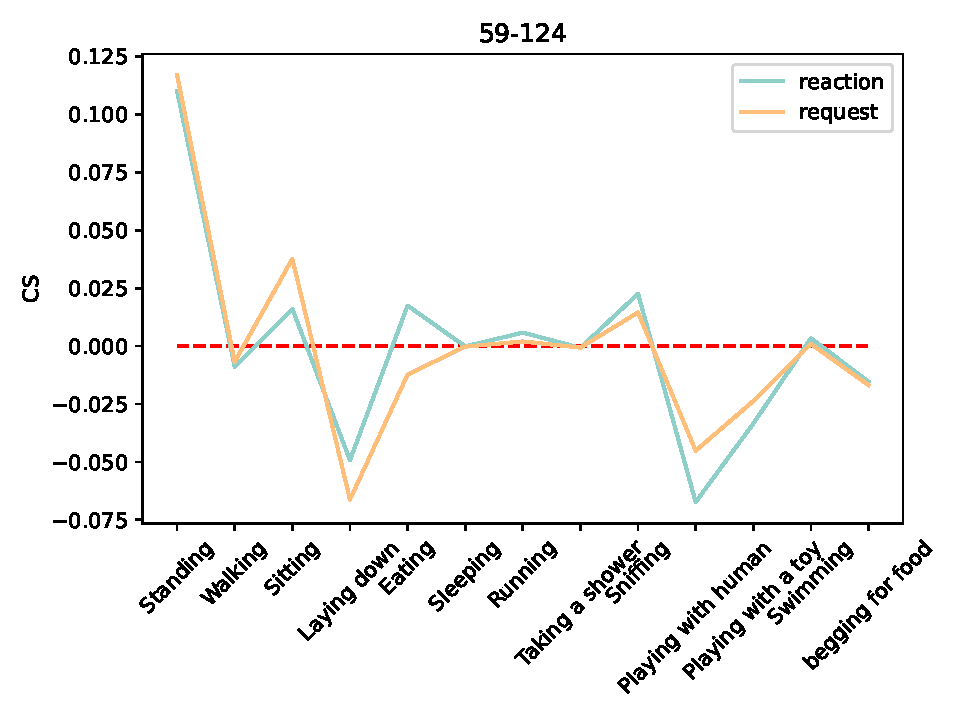
\includegraphics[width=0.99\linewidth]{./35word/59-124.pdf}
		\end{minipage}
		\begin{minipage}[b]{.3\linewidth}
			\centering
			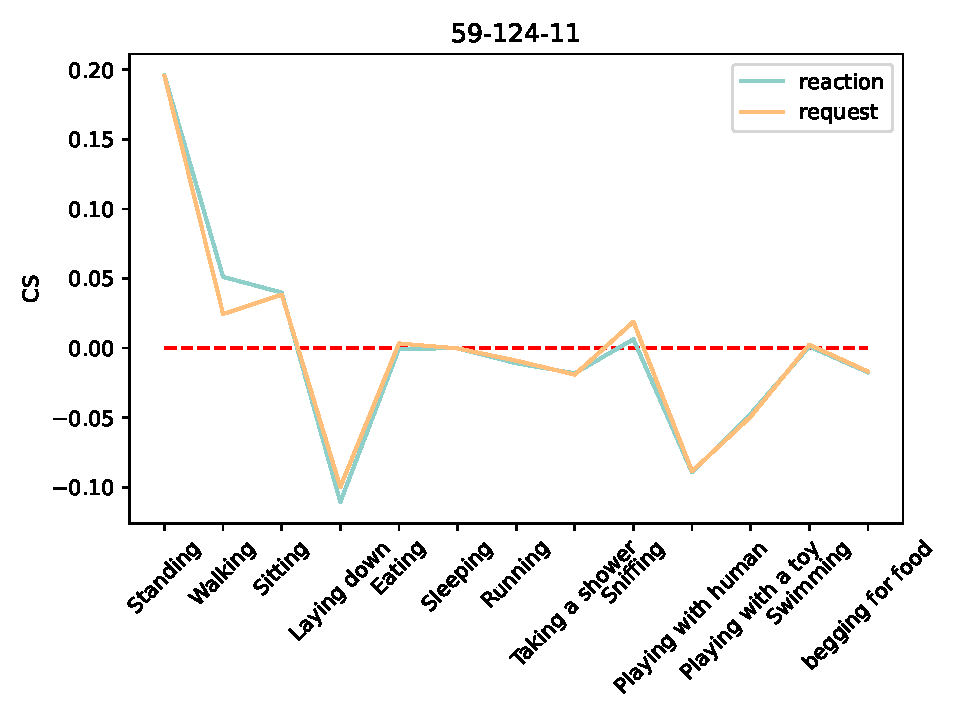
\includegraphics[width=0.99\linewidth]{./35word/59-124-11.pdf}
		\end{minipage}
		\begin{minipage}[b]{.3\linewidth}
			\centering
			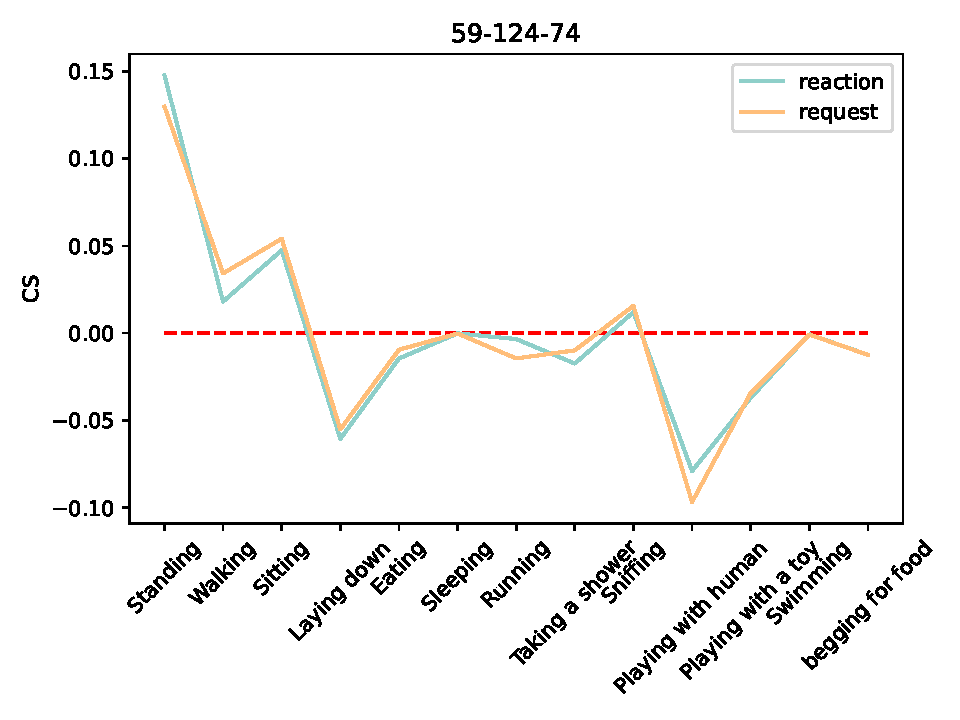
\includegraphics[width=0.99\linewidth]{./35word/59-124-74.pdf}
		\end{minipage}
		
%				\begin{minipage}[b]{.3\linewidth}
%			\centering
%			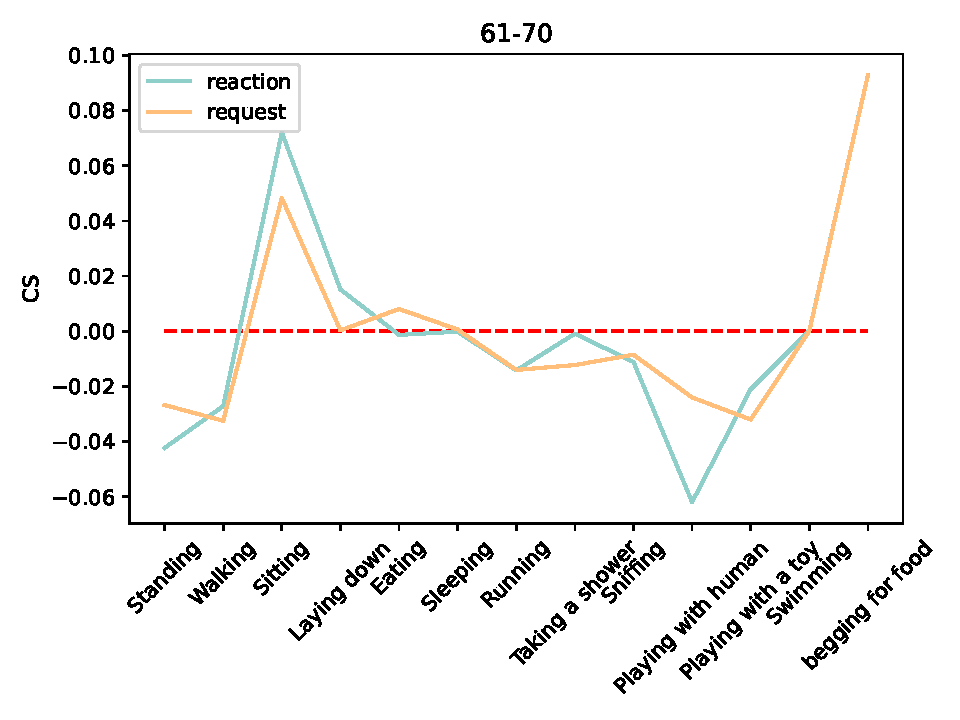
\includegraphics[width=0.99\linewidth]{./35word/61-70.pdf}
%		\end{minipage}
%		\begin{minipage}[b]{.3\linewidth}
%			\centering
%			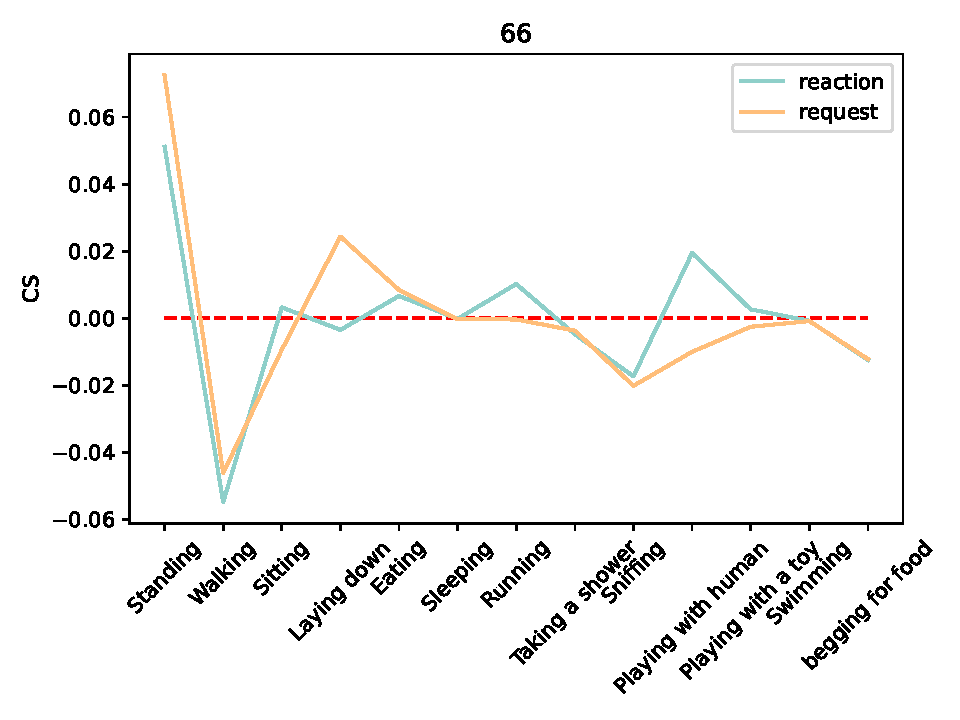
\includegraphics[width=0.99\linewidth]{./35word/66.pdf}
%		\end{minipage}
%		\begin{minipage}[b]{.3\linewidth}
%			\centering
%			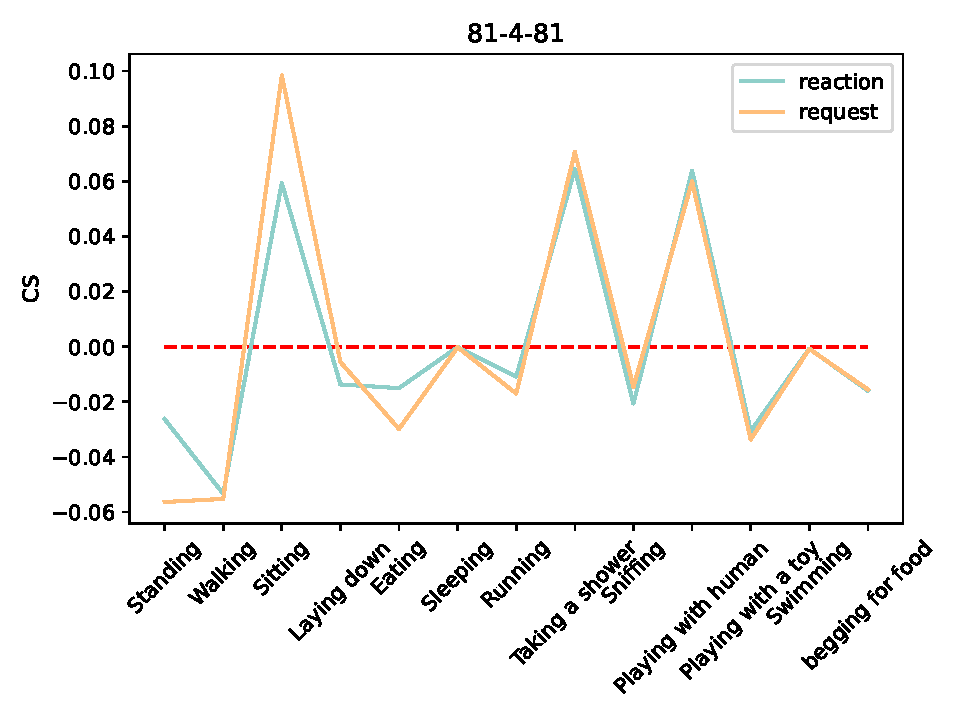
\includegraphics[width=0.99\linewidth]{./35word/81-4-81.pdf}
%		\end{minipage}
%%%%%%%%%%%%%%%%%%
	\caption{Causal strength of top 35 words~(part 1).}
		\label{fig:words35p1}
\end{figure*}

\begin{figure*}[ht]
		\centering
%	\ContinuedFloat
					\begin{minipage}[b]{.3\linewidth}
		\centering
		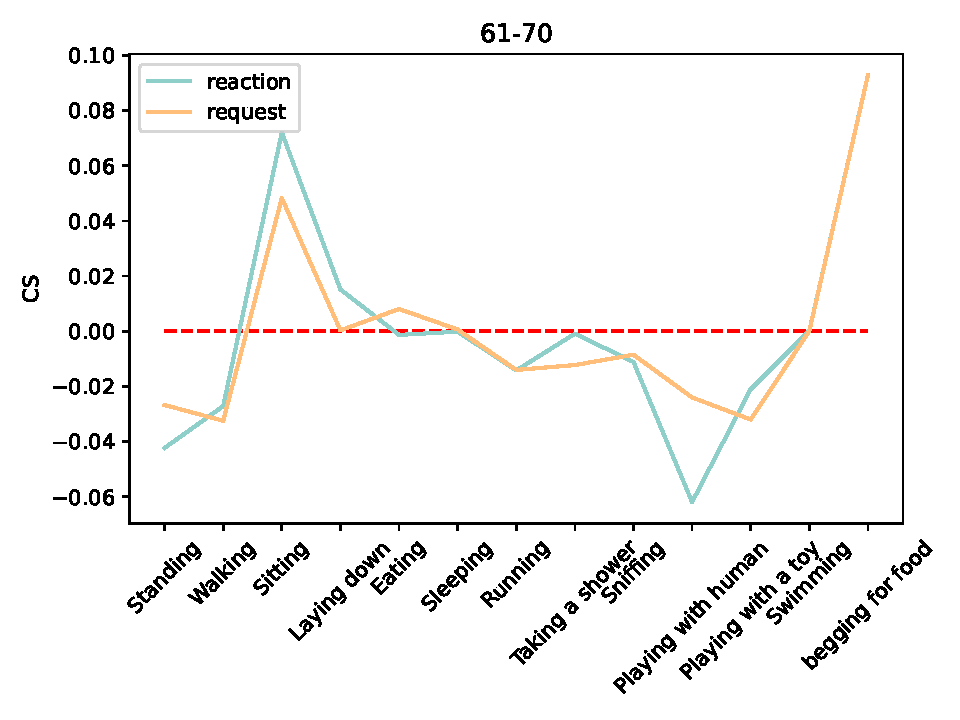
\includegraphics[width=0.99\linewidth]{./35word/61-70.pdf}
	\end{minipage}
	\begin{minipage}[b]{.3\linewidth}
		\centering
		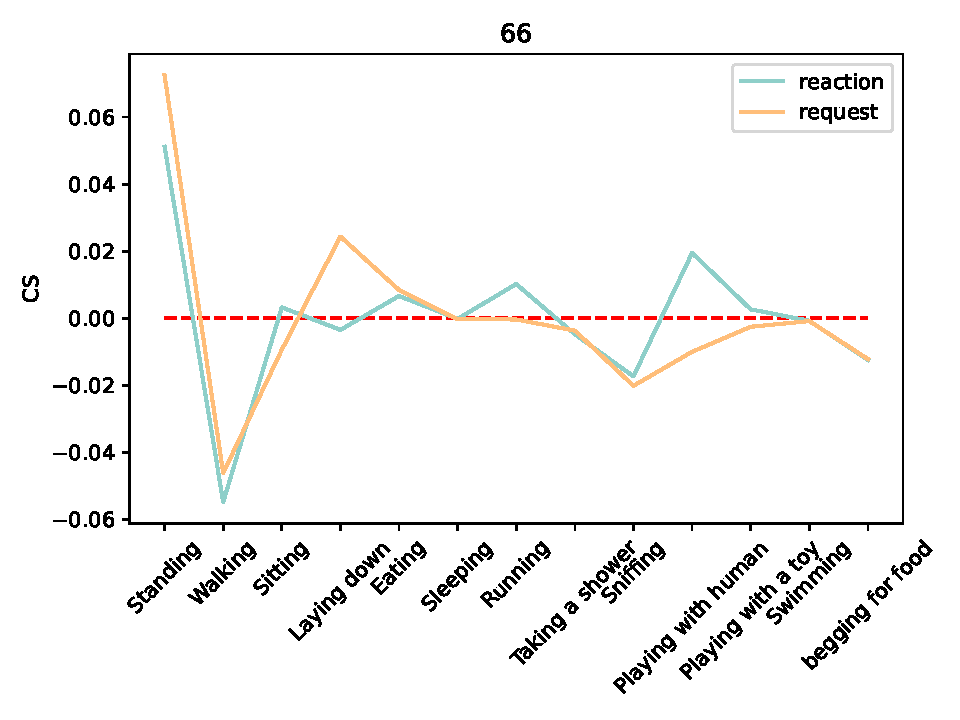
\includegraphics[width=0.99\linewidth]{./35word/66.pdf}
	\end{minipage}
	\begin{minipage}[b]{.3\linewidth}
		\centering
		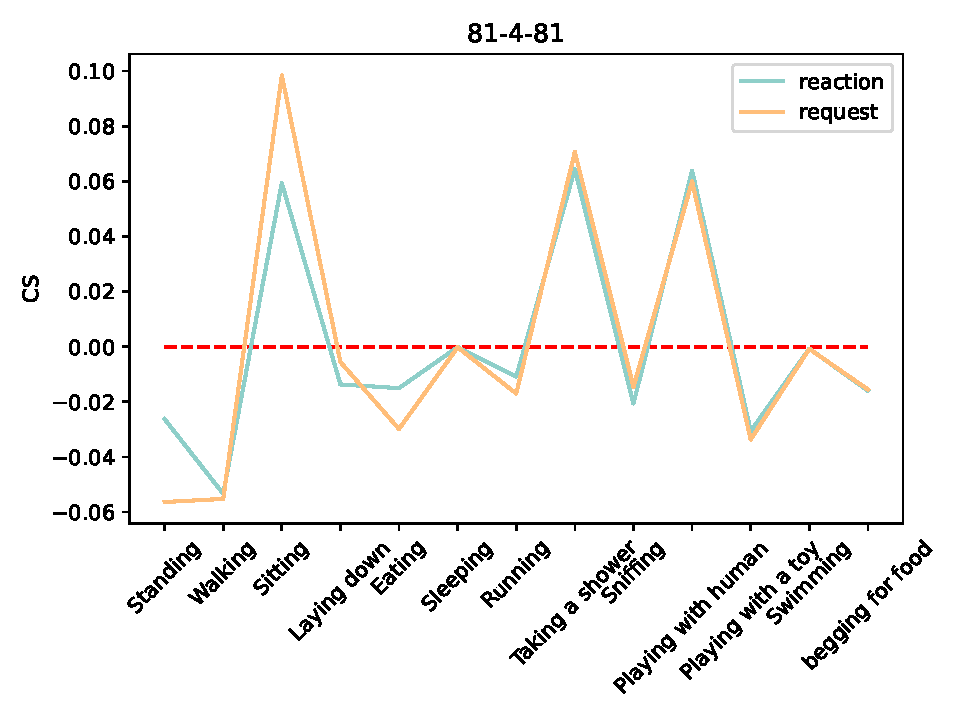
\includegraphics[width=0.99\linewidth]{./35word/81-4-81.pdf}
	\end{minipage}
	
		\begin{minipage}[b]{.3\linewidth}
			\centering
			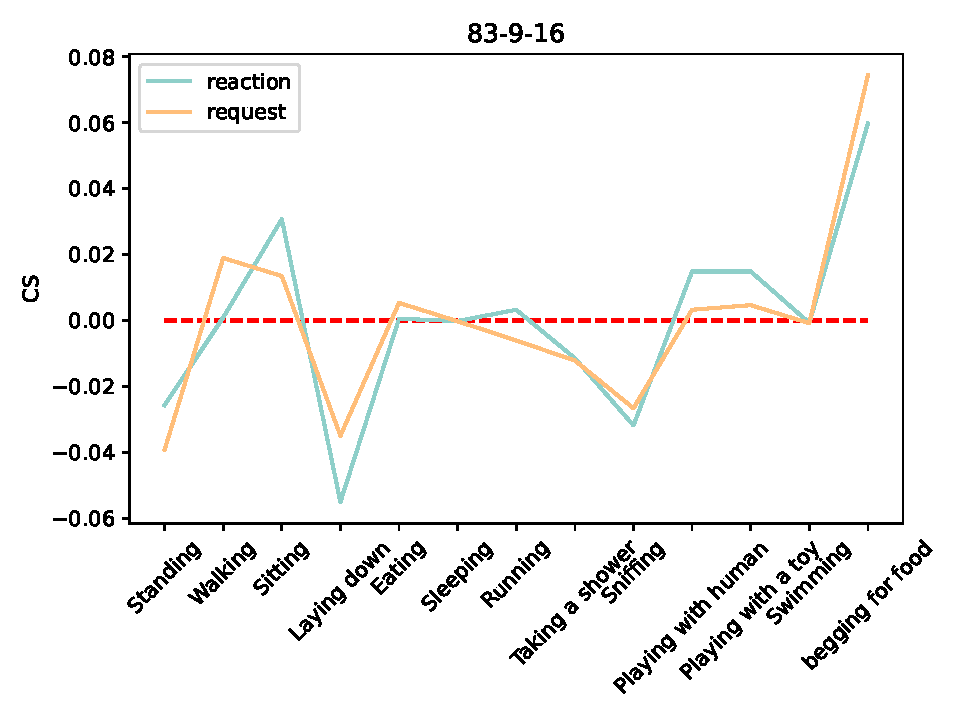
\includegraphics[width=0.99\linewidth]{./35word/83-9-16.pdf}
		\end{minipage}
		\begin{minipage}[b]{.3\linewidth}
			\centering
			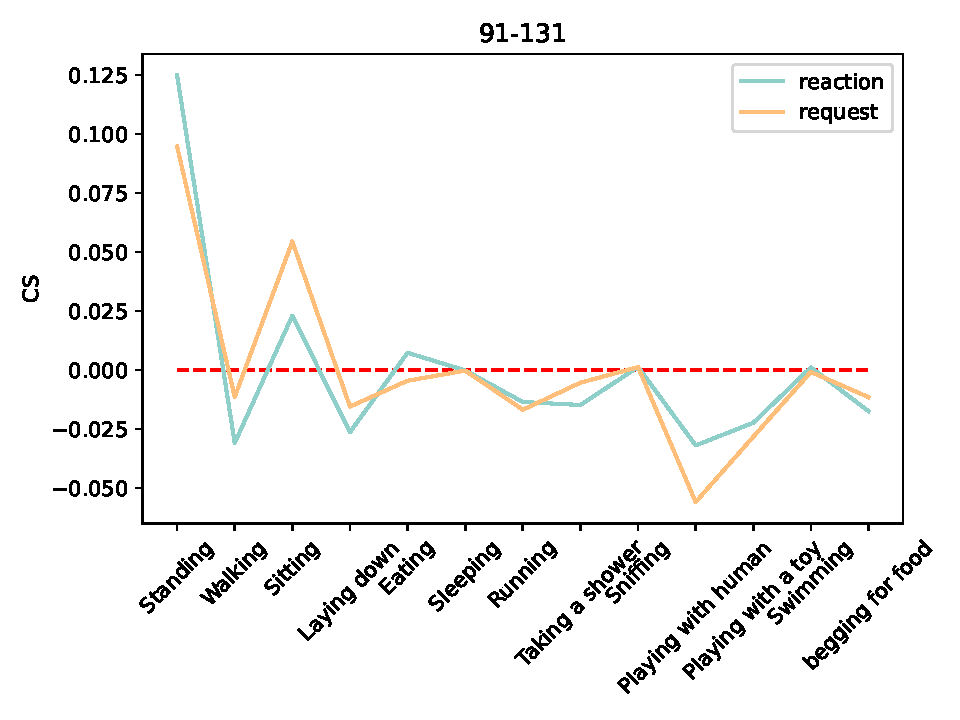
\includegraphics[width=0.99\linewidth]{./35word/91-131.pdf}
		\end{minipage}
		\begin{minipage}[b]{.3\linewidth}
			\centering
			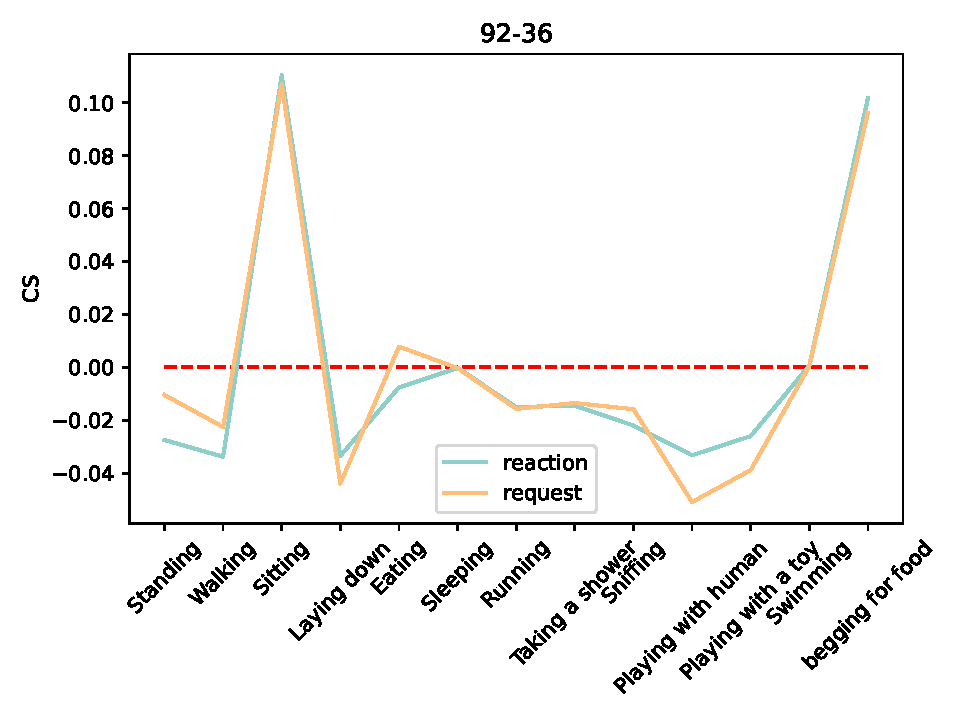
\includegraphics[width=0.99\linewidth]{./35word/92-36.pdf}
		\end{minipage}
		
				\begin{minipage}[b]{.3\linewidth}
			\centering
			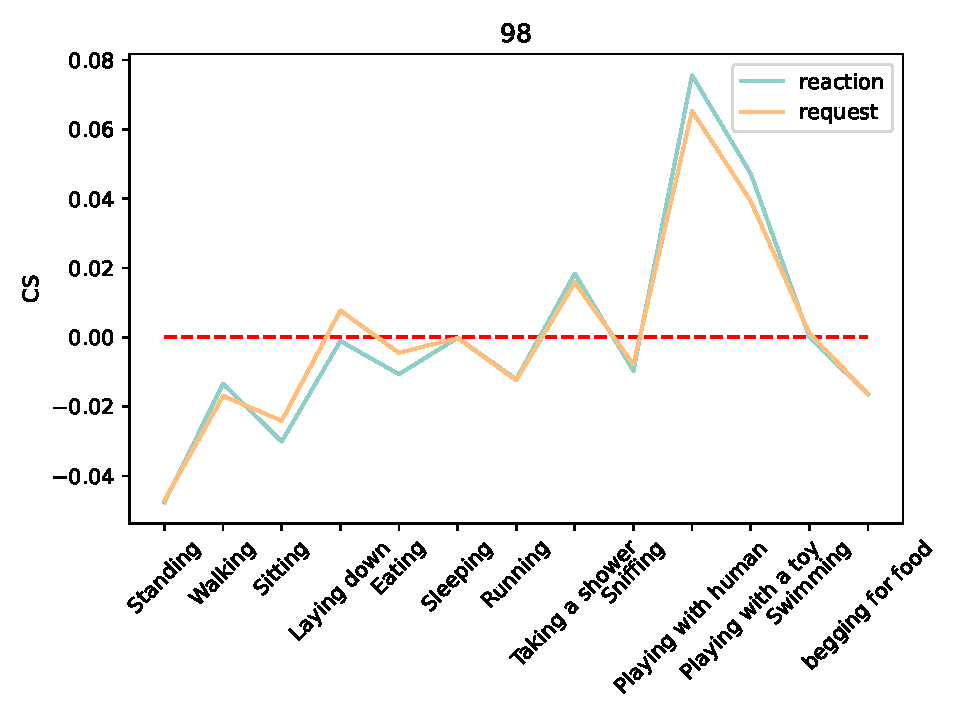
\includegraphics[width=0.99\linewidth]{./35word/98.pdf}
		\end{minipage}
		\begin{minipage}[b]{.3\linewidth}
			\centering
			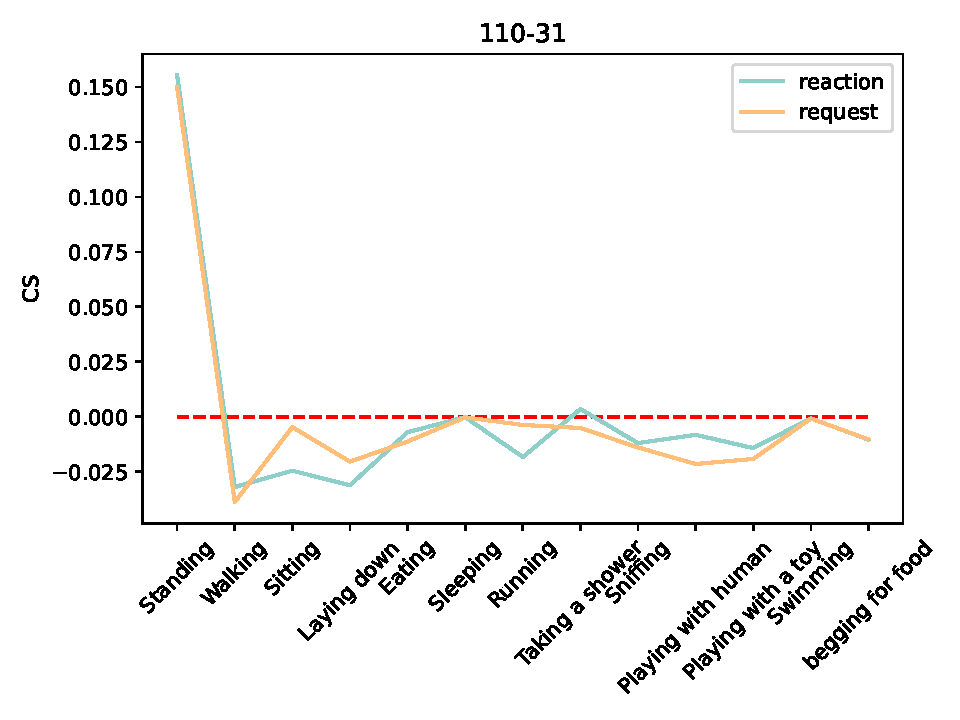
\includegraphics[width=0.99\linewidth]{./35word/110-31.pdf}
		\end{minipage}
		\begin{minipage}[b]{.3\linewidth}
			\centering
			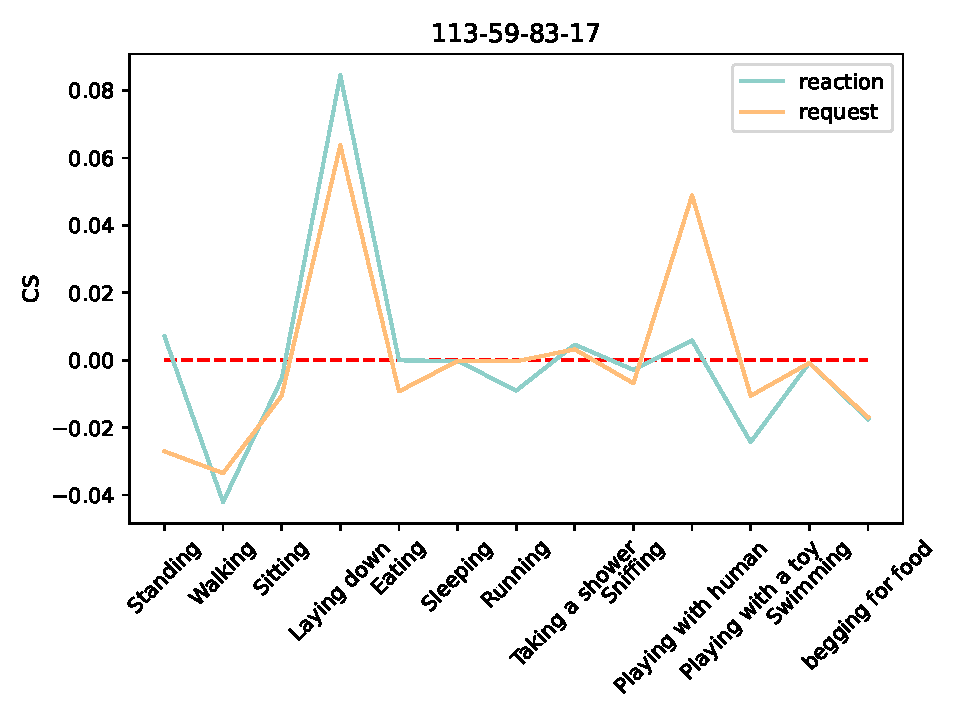
\includegraphics[width=0.99\linewidth]{./35word/113-59-83-17.pdf}
		\end{minipage}
		
		\begin{minipage}[b]{.3\linewidth}
			\centering
			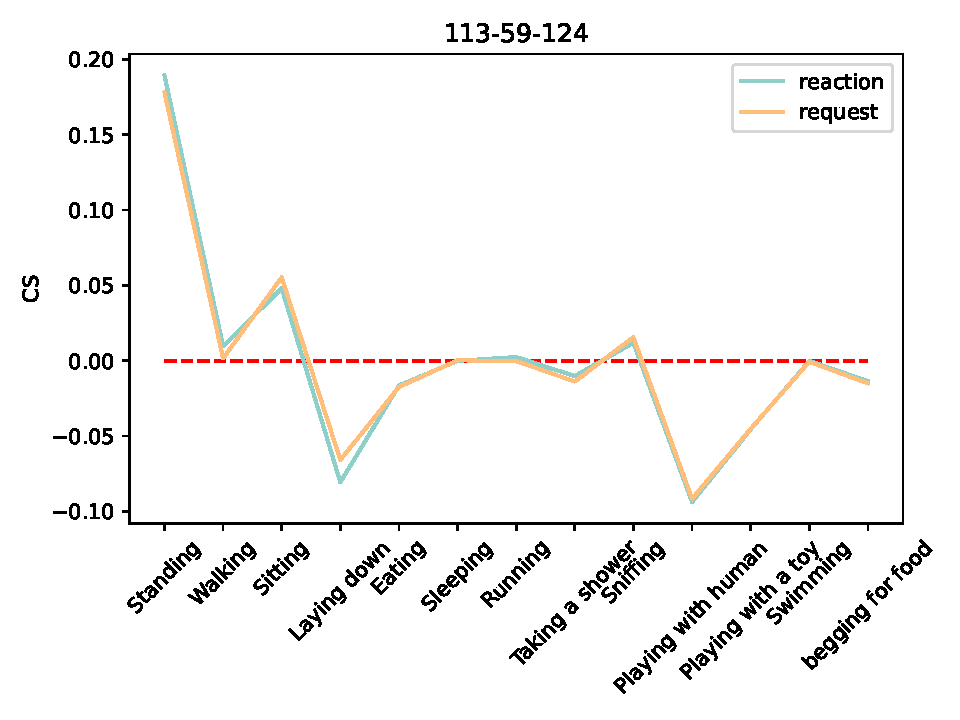
\includegraphics[width=0.99\linewidth]{./35word/113-59-124.pdf}
		\end{minipage}
		\begin{minipage}[b]{.3\linewidth}
			\centering
			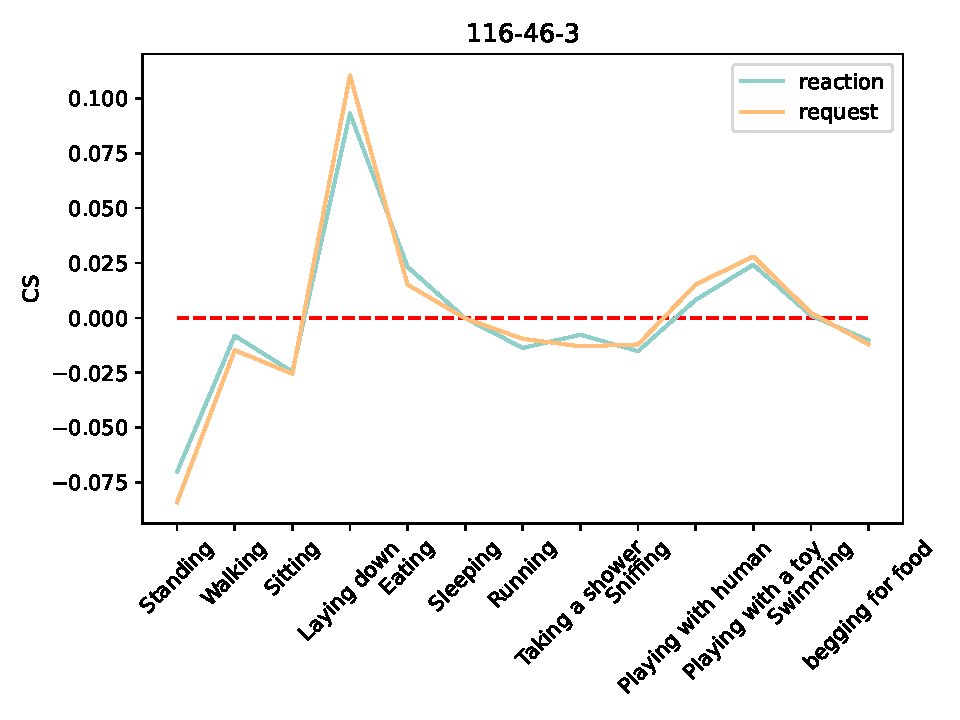
\includegraphics[width=0.99\linewidth]{./35word/116-46-3.pdf}
		\end{minipage}
		\begin{minipage}[b]{.3\linewidth}
			\centering
			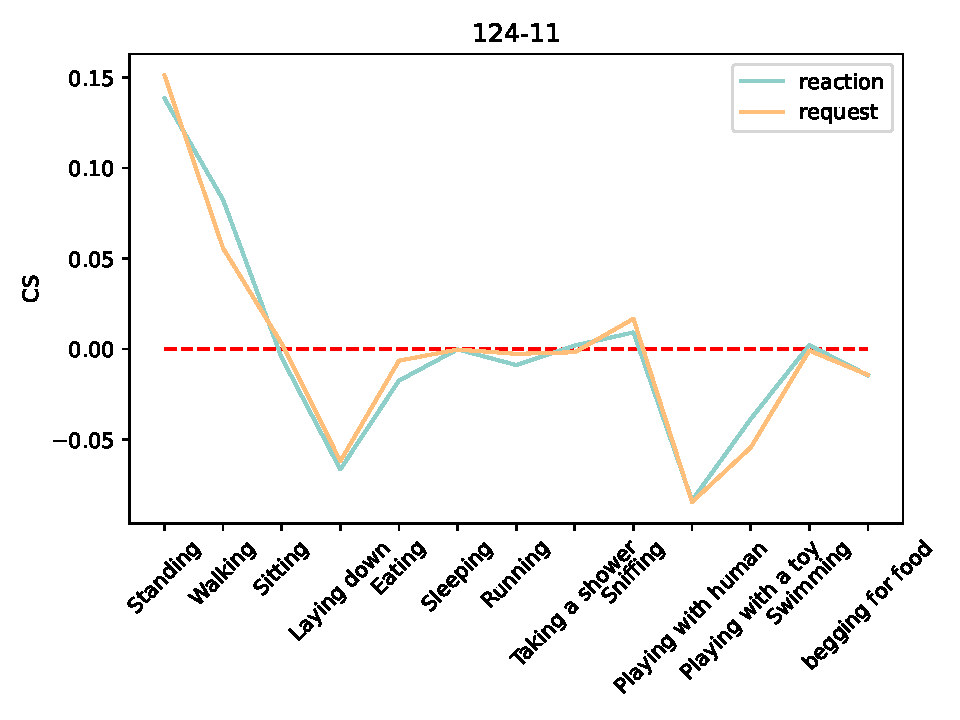
\includegraphics[width=0.99\linewidth]{./35word/124-11.pdf}
		\end{minipage}
		
				\begin{minipage}[b]{.3\linewidth}
			\centering
			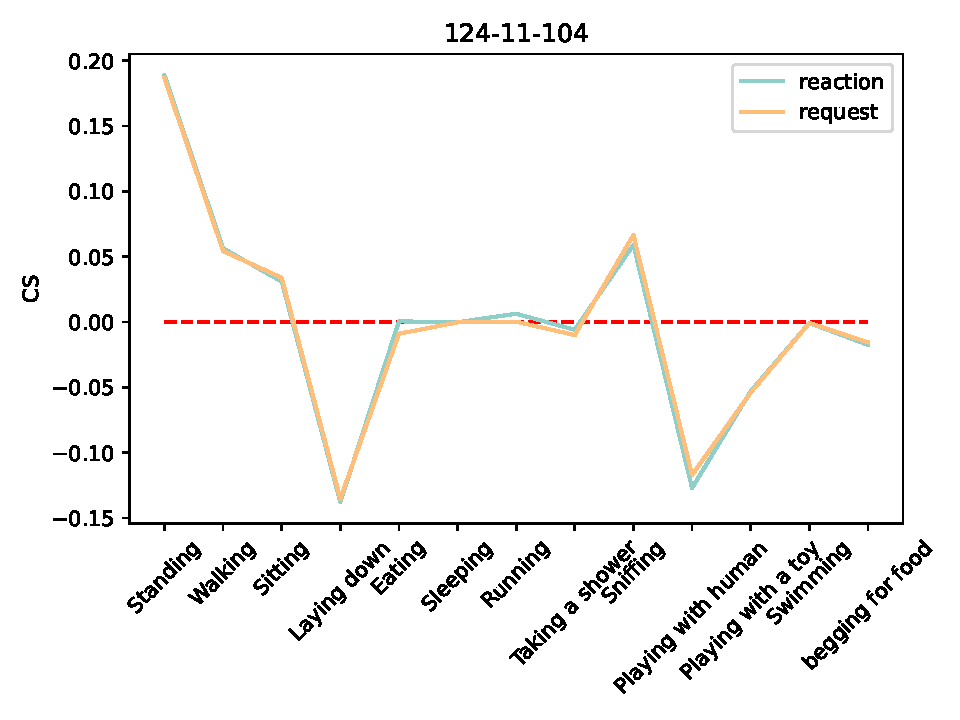
\includegraphics[width=0.99\linewidth]{./35word/124-11-104.pdf}
		\end{minipage}
		\begin{minipage}[b]{.3\linewidth}
			\centering
			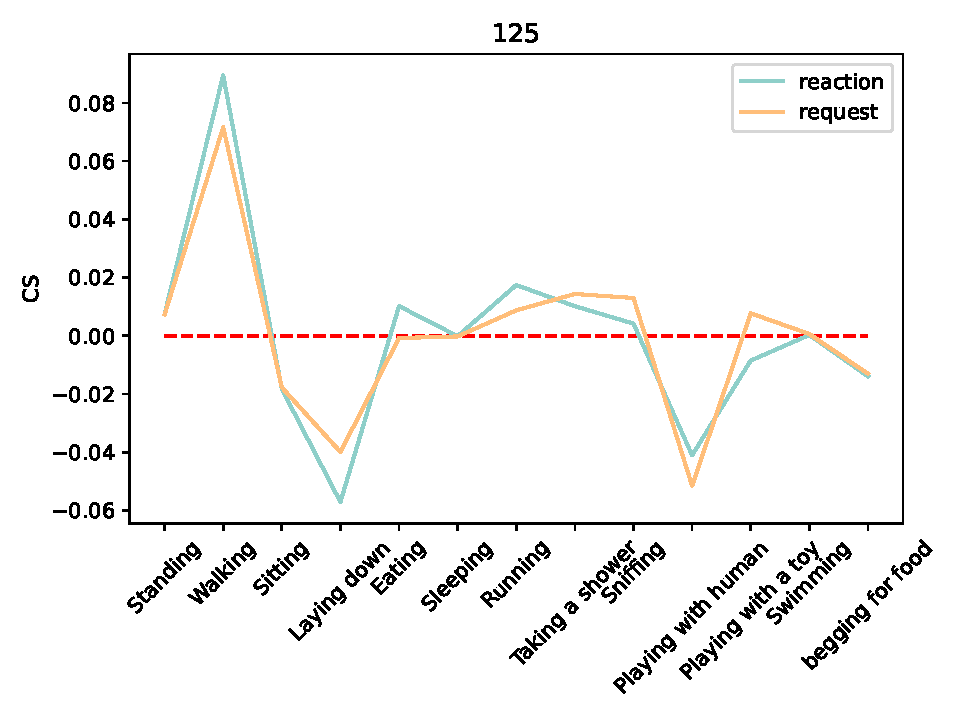
\includegraphics[width=0.99\linewidth]{./35word/125.pdf}
		\end{minipage}
		\begin{minipage}[b]{.3\linewidth}
			\centering
			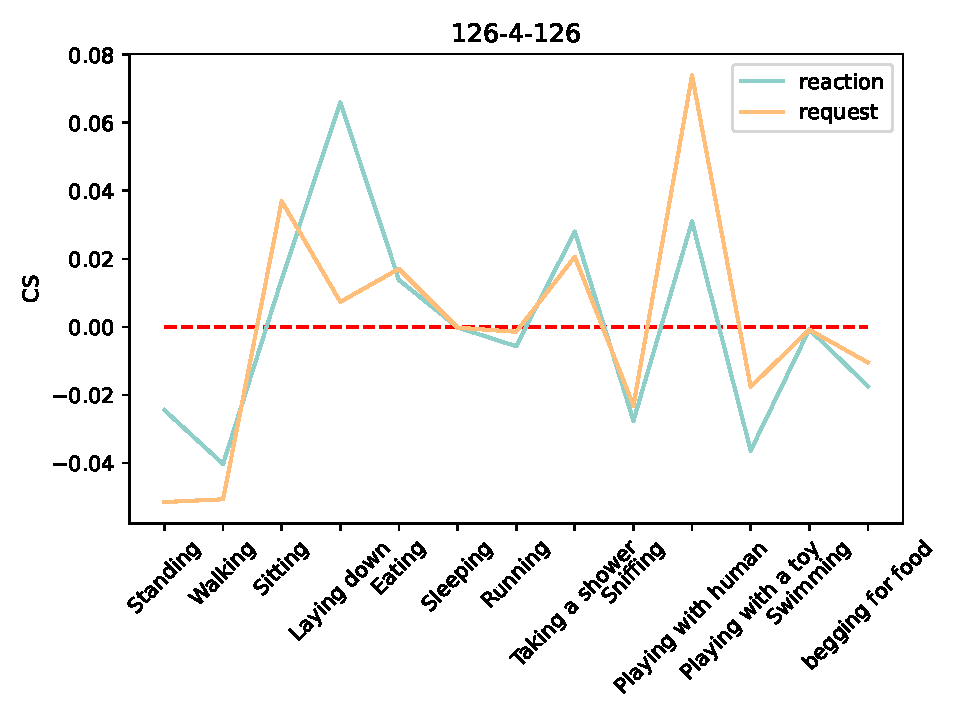
\includegraphics[width=0.99\linewidth]{./35word/126-4-126.pdf}
		\end{minipage}
		
		\begin{minipage}[b]{.3\linewidth}
			\centering
			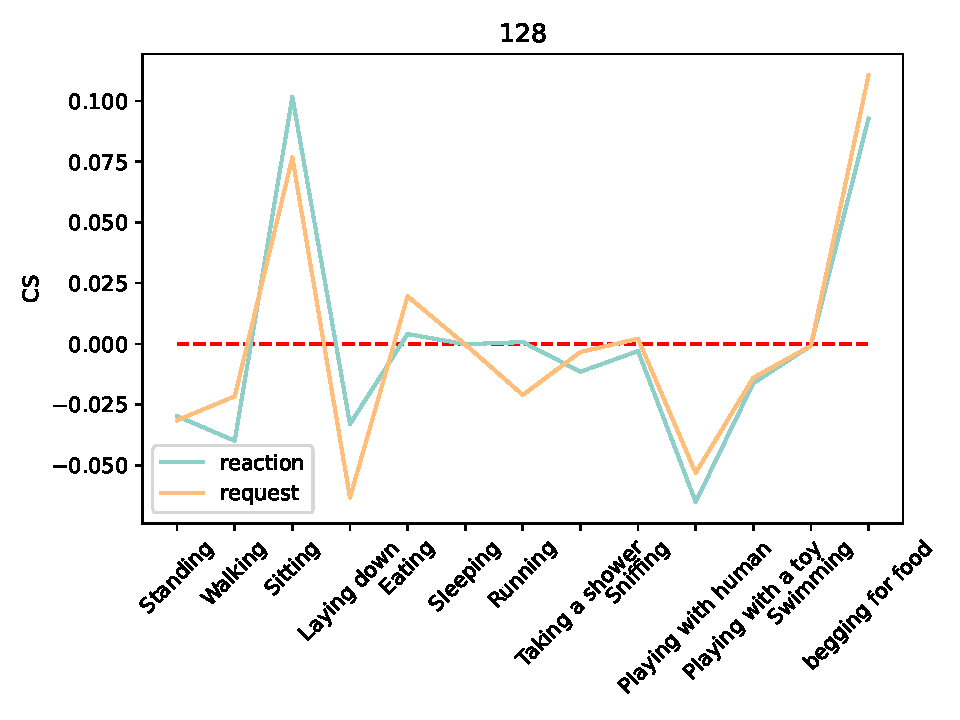
\includegraphics[width=0.99\linewidth]{./35word/128.pdf}
		\end{minipage}
		\begin{minipage}[b]{.3\linewidth}
			\centering
			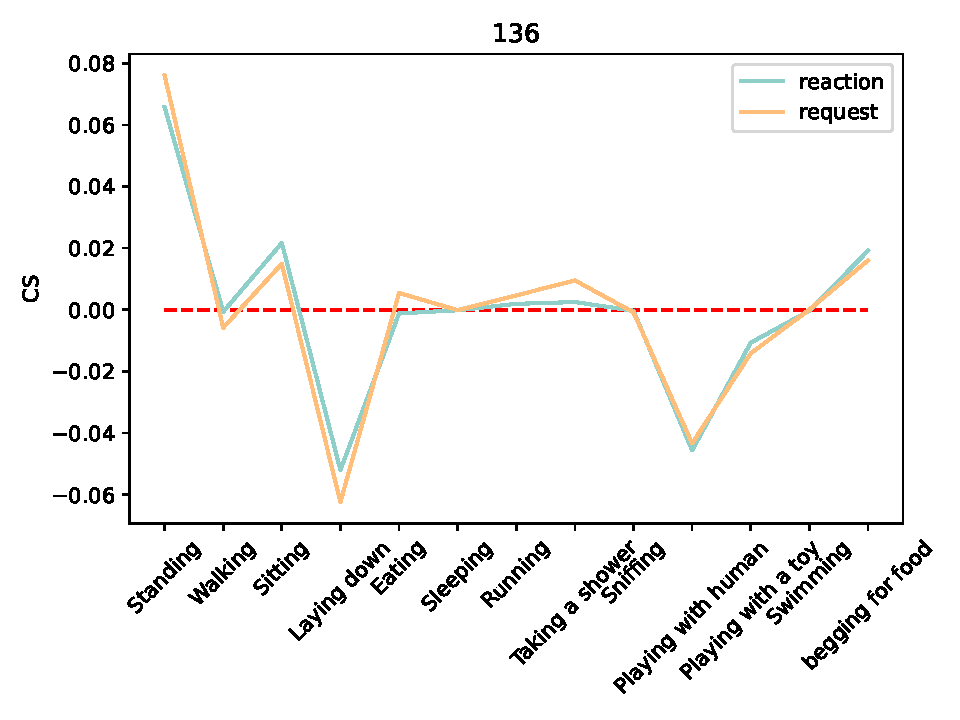
\includegraphics[width=0.99\linewidth]{./35word/136.pdf}
		\end{minipage}

	\caption{Causal strength of top 35 words~(part 2).}
	\label{fig:words35p2}
\end{figure*}
